\chapter{Lab 9 - Filters}

%%%%%%%%%%%%%%%%%%%%%%%%%%%%%%%%%%%%%%%%%%%%%%%%%%%%%%%%%%%%%%%%%%%%%%%%%%%%%%%%%%%%%%%%%%%%%%%%%%%%%%%
\section{Objective}
%%%%%%%%%%%%%%%%%%%%%%%%%%%%%%%%%%%%%%%%%%%%%%%%%%%%%%%%%%%%%%%%%%%%%%%%%%%%%%%%%%%%%%%%%%%%%%%%%%%%%%%

The objective of this lab is to introduce the concept of filters and explore their applications through examples of passive and active filters. 

%%%%%%%%%%%%%%%%%%%%%%%%%%%%%%%%%%%%%%%%%%%%%%%%%%%%%%%%%%%%%%%%%%%%%%%%%%%%%%%%%%%%%%%%%%%%%%%%%%%%%%
\section{Materials}
%%%%%%%%%%%%%%%%%%%%%%%%%%%%%%%%%%%%%%%%%%%%%%%%%%%%%%%%%%%%%%%%%%%%%%%%%%%%%%%%%%%%%%%%%%%%%%%%%%%%%%%

\begin{itemize}
	\item Laptop with LTSpice
	\item Analog Discovery
	\item Breadboard
	\item Wiring kit
	\item Lab parts kit
\end{itemize}

%%%%%%%%%%%%%%%%%%%%%%%%%%%%%%%%%%%%%%%%%%%%%%%%%%%%%%%%%%%%%%%%%%%%%%%%%%%%%%%%%%%%%%%%%%%%%%%%%%%%%%%
\section{Introduction}
%%%%%%%%%%%%%%%%%%%%%%%%%%%%%%%%%%%%%%%%%%%%%%%%%%%%%%%%%%%%%%%%%%%%%%%%%%%%%%%%%%%%%%%%%%%%%%%%%%%%%%%

Laboratories so far have focused on the time domain. Given a signal with a specific frequency, there is a resulting output that can be viewed with an appropriate time base on the o-scope. Filters are analyzed primary through the frequency domain, where the output is a function of frequency and not time. 

Filters, as the name implies, filters out certain frequencies from passing to the output. There are several types of filters, such lowpass, highpass, bandpass, notch (bandreject), and allpass. While there are applications for all the filter types, there is only enough time to focus on a few, in this case, lowpass and highpass. Additionally, the math associated with filters can become complicated quickly and so only the results will be represented here. 

\begin{figure}
	\centering
		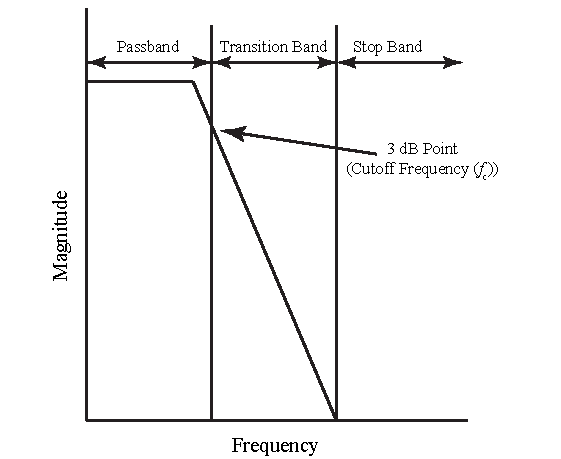
\includegraphics[width=0.5\textwidth]{Lab7FilterResponse.pdf}
	\caption{Example of response for a generic lowpass filter. The filter passes low frequencies frequencies, thus the name, and attenuates higher frequencies. } \label{fig:filterResponse}
\end{figure}

\hyperref[fig:filterResponse]{Figure \ref*{fig:filterResponse}} is an example of a generic lowpass filter response in the frequency domain. The filter, as the name implies, will only pass low frequency signals, higher frequency signals are attenuated through the transition and stop bands. A filter's 3 dB point, cut off frequency, is set by design and is often chosen to obtain a specific attenuation at a certain frequency. Similarly, a high pass filter will behave in the opposite fashion, low frequency signals will be attenuated while high frequency signals will be passed. 

%%%%%%%%%%%%%%%%%%%%%%%%%%%%%%%%%%%%%%%%%%%%%%%%%%%%%%%%%%%%%%%%%%%%%%%%%%%%%%%%%%%%%%%%%%%%%%%%%%%%%%%
\subsection{Passive First Order RC Filters}
%%%%%%%%%%%%%%%%%%%%%%%%%%%%%%%%%%%%%%%%%%%%%%%%%%%%%%%%%%%%%%%%%%%%%%%%%%%%%%%%%%%%%%%%%%%%%%%%%%%%%%%

\hyperref[fig:simpleRC]{Figure \ref*{fig:simpleRC}} shows two simple RC filter configurations and their resulting frequency responses. These filters are considered to be passive, no active elements that require power, and of the first order, there's only one combination of resistors and capacitors. 

\begin{figure}[h]
	\centering
		\includegraphics[width=1\textwidth]{Lab9RCFilters.pdf}
	\caption{An example of a simple RC low pass filter (a) and the resulting frequency response (b). Also, a simple RC highpass filter (c) and the resulting frequency response (d).} \label{fig:simpleRC}
\end{figure}

While the configurations may seem puzzling at first, their results come easily when considering the effects at low and high frequencies. At low frequency, a capacitor acts as an open circuit, $\frac{1}{j\omega C}$ is large when $\omega =2\pi f$ is small, while at high frequencies, it acts as a short circuit, $\frac{1}{j\omega C}$ is small when $\omega$ is large. So, for a lowpass, it makes sense that low frequencies are passed while high frequencies are attenuated. Similarly, for a highpass filter, low frequencies are attenuated while high frequencies are passed. 

There are a variety of equations relating the transfer function of a filter, but instead the focus is on the important parameters. In the case of a simple RC filter, the 3 dB point, or the frequency where the output has dropped to half of the input, is governed by the following equation:

\begin{equation}
f_c = \frac{1}{2 \pi RC}
\end{equation}

\noindent For the examples in \hyperref[fig:simpleRC]{Figure \ref*{fig:simpleRC} (a) and (c)}, the 3 dB point is calculated to be $\frac{1}{2 \pi 10\mathrm{k}\; 0.001\mu} = 15.916\;\mathrm{kHz}$. Which matches the frequency response for both configurations. 

%%%%%%%%%%%%%%%%%%%%%%%%%%%%%%%%%%%%%%%%%%%%%%%%%%%%%%%%%%%%%%%%%%%%%%%%%%%%%%%%%%%%%%%%%%%%%%%%%%%%%%%
\subsection{Active RC Filters}
%%%%%%%%%%%%%%%%%%%%%%%%%%%%%%%%%%%%%%%%%%%%%%%%%%%%%%%%%%%%%%%%%%%%%%%%%%%%%%%%%%%%%%%%%%%%%%%%%%%%%%%

There are a variety of active filter topologies but a simple implementation is to use an appropriately placed capacitor in conjunction with a typical inverting amplifier configuration, \hyperref[fig:9activeRC]{Figure \ref*{fig:9activeRC} (a) and (b)}.

\begin{figure}[h]
	\centering
		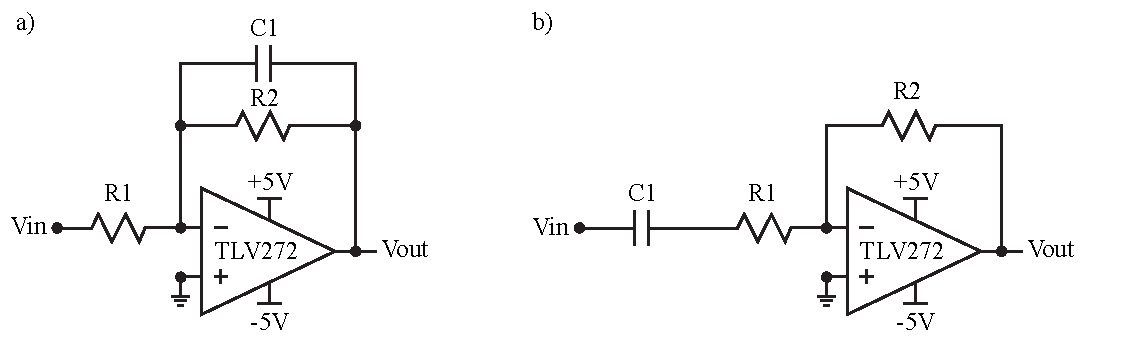
\includegraphics[width=1\textwidth]{Lab9activeRC.pdf}
	\caption{An example of an active RC low pass filter (a) and an active RC high pass filter (b).} \label{fig:9activeRC}
\end{figure}

The design of either the active RC low pass or high pass is also fairly simple for the first order case. A low pass filter has the following equations

\begin{align*}
	\frac{V_{OUT}}{V_{IN}} &= -\frac{R_2}{R_1}\frac{1}{j\omega C_1 R_2 +1} \\
	H_0 &= -\frac{R_2}{R_1} \\
	f_0 &= \frac{1}{2 \pi C_1 R_2} \\
\end{align*}

\noindent where $H_0$ is the passband gain and $f_0$ is the 3dB frequency. Note that unlike the passive RC case, filters using op amps can also have gain. Similarly, the high pass filter has the following equations

\begin{align*}
	\frac{V_{OUT}}{V_{IN}} &= -\frac{R_2}{R_1}\frac{j\omega C_1 R_1}{j\omega C_1 R_1 +1}\\ 
	H_0 &= -\frac{R_2}{R_1}\\
	f_0 &= \frac{1}{2 \pi C_1 R_1}\\
\end{align*}


%%%%%%%%%%%%%%%%%%%%%%%%%%%%%%%%%%%%%%%%%%%%%%%%%%%%%%%%%%%%%%%%%%%%%%%%%%%%%%%%%%%%%%%%%%%%%%%%%%%%%%%%
%\subsection{Active RC Filters - Sallen-Key}
%%%%%%%%%%%%%%%%%%%%%%%%%%%%%%%%%%%%%%%%%%%%%%%%%%%%%%%%%%%%%%%%%%%%%%%%%%%%%%%%%%%%%%%%%%%%%%%%%%%%%%%%
%
%There are a variety of active filter oligopolies but one of the most poplar is the Sallen-Key topology, named after R. P. Sallen and E. L. Key, because the filter depends on the external components and not the op amp. \hyperref[fig:sallenKey]{Figure \ref*{fig:sallenKey}} shows the lowpass and highpass configurations. 
%
%\begin{figure}
	%\centering
		%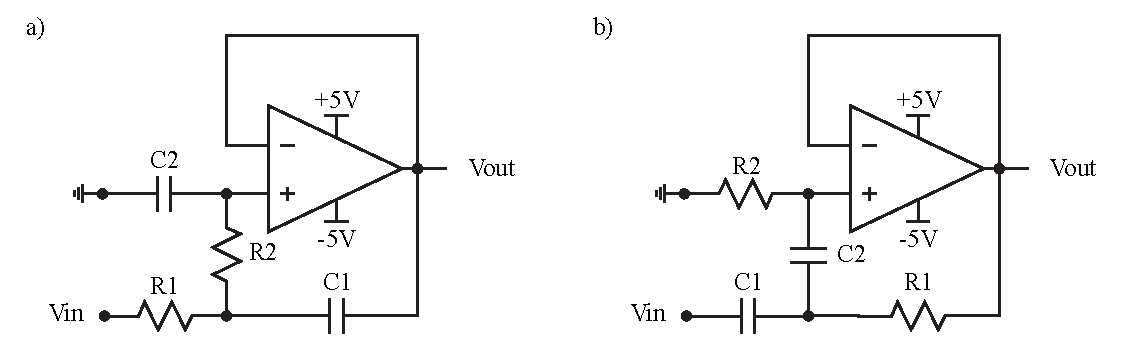
\includegraphics[width=1\textwidth]{lab7sallenkey.pdf}
	%\caption{A Sallen-Key lowpass filter (a) and highpass (b). Note that this is a simplified topology with unity gain.} \label{fig:sallenKey}
%\end{figure}
%
%The design of this filter is more complicated than the simple RC and requires a bit of foresight. For a lowpass, choose C1 and then calculated the other values using the following coefficients and equations
%
%\begin{subequations}
%\	\begin{align}
		%k &= 2\pi f_0 C_1 \\
		%m &= \frac{\alpha^2}{4} \\
		%C_2 &= m C_1 \\
		%R_1 &= \frac{2}{\alpha k} \\
		%R_2 &= \frac{\alpha}{2 m k} 
	%\end{align}
%\end{subequations}
%
%\noindent where $f_0$ is the desired 3 dB point in Hz and $\alpha = 1.4142$ for a second order filter. If the desired $f_0$ is 10 kHz and C1 is chosen to be $0.01\; \mu$F, the remaining values are C2 = $0.005\;\mu$F and R1 = R2 = 2.25 k$\Omega$.
%
%The design equations for a Sallen-Key highpass are similar:
%
%\begin{subequations}
%\	\begin{align}
		%k &= 2\pi f_0 C_1 \\
		%C_2 &= C_1 \\
		%R_1 &= \frac{2\alpha}{4k} \\
		%R_2 &= \frac{4}{2\alpha}\frac{1}{k}
	%\end{align}
%\end{subequations}
%
%\noindent where $f_0$ is the desired 3 dB point in Hz and $\alpha = 1.4142$ for a second order filter. Consider a similar design where $f_0$ is 10 kHz and C1 is chosen to be $0.01\; \mu$F, the remaining values are C2 = $0.01\; \mu$F and R1 = 1.25 k$\Omega$ and R2 = 2.25 k$\Omega$.

%%%%%%%%%%%%%%%%%%%%%%%%%%%%%%%%%%%%%%%%%%%%%%%%%%%%%%%%%%%%%%%%%%%%%%%%%%%%%%%%%%%%%%%%%%%%%%%%%%%%%%%
\section{Big Picture}
%%%%%%%%%%%%%%%%%%%%%%%%%%%%%%%%%%%%%%%%%%%%%%%%%%%%%%%%%%%%%%%%%%%%%%%%%%%%%%%%%%%%%%%%%%%%%%%%%%%%%%%

\begin{figure} [h]
	\centering
		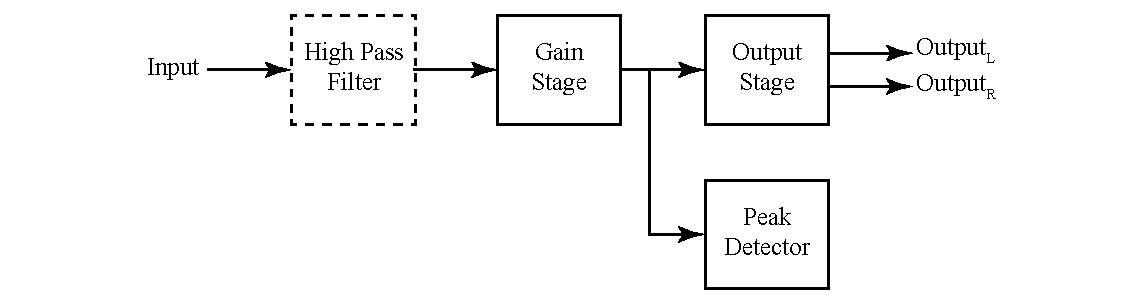
\includegraphics[width=1\textwidth]{Lab9bigpicture.pdf}
	\caption{Big picture with emphasis on the high pass filter.} \label{fig:9bp}
\end{figure}

This lab focuses on filter circuits which will help to create the high pass filter used in the final project used to remove the large DC offset in the source signal. 

%%%%%%%%%%%%%%%%%%%%%%%%%%%%%%%%%%%%%%%%%%%%%%%%%%%%%%%%%%%%%%%%%%%%%%%%%%%%%%%%%%%%%%%%%%%%%%%%%%%%%%%
\section{Pre-Lab Requirements}
%%%%%%%%%%%%%%%%%%%%%%%%%%%%%%%%%%%%%%%%%%%%%%%%%%%%%%%%%%%%%%%%%%%%%%%%%%%%%%%%%%%%%%%%%%%%%%%%%%%%%%%

Complete the following before coming to lab. 

%%%%%%%%%%%%%%%%%%%%%%%%%%%%%%%%%%%%%%%%%%%%%%%%%%%%%%%%%%%%%%%%%%%%%%%%%%%%%%%%%%%%%%%%%%%%%%%%%%%%%%%
\subsection{LTspice Simulations} \label{ssec:9spice}
%%%%%%%%%%%%%%%%%%%%%%%%%%%%%%%%%%%%%%%%%%%%%%%%%%%%%%%%%%%%%%%%%%%%%%%%%%%%%%%%%%%%%%%%%%%%%%%%%%%%%%%

Complete the following using the TLV271 spice model, always power the op amp with +/- 5 V for $V_{dd+}$ and $V_{dd-}$.

\begin{enumerate}
\item Review the LTspice tutorial for AC Analysis, \url{https://www.youtube.com/watch?v=fziUQaVQxA4&t=1s}.
	\item Build a simple lowpass filter, \hyperref[fig:simpleRC]{Figure \ref*{fig:simpleRC} (a)}, but set R = 10 k$\Omega$ and C = $0.001\; \mu$F. Set the voltage source to an AC amplitude of 1 and run an AC analysis with the following settings: Decade, 100, 1, 1Meg. Save an image of the circuit, a plot of the output, and table the 3 dB frequency for submission to Canvas. \label{itm:9ssec1itm1}
	\item Build a simple highpass filter, \hyperref[fig:simpleRC]{Figure \ref*{fig:simpleRC} (c)}, but set R = 15 k$\Omega$ and C = $0.01\; \mu$F. Set the voltage source to an AC amplitude of 1 and run an AC analysis with the following settings: Decade, 100, 1, 1Meg. Save an image of the circuit, a plot of the output, and table the 3 dB frequency for submission to Canvas. \label{itm:9ssec1itm2}
	\item Build an active RC lowpass filter, \hyperref[fig:9activeRC]{Figure \ref*{fig:9activeRC} (a)}. Set $C_1 = 0.1\mu$F and determine the resistor values for a gain of -1 V/V (0 dB) and a $f_0 = 1.59\;\mathrm{kHz}$ using only values in your lab kit. Set the voltage source to an AC amplitude of 1 and run an AC analysis with the following settings: Decade, 100, 1, 1Meg. Save an image of the circuit, a plot of the output, and table the 3 dB frequency for submission to Canvas. \label{itm:9ssec1itm3}
	\item Build an active RC highpass filter, \hyperref[fig:9activeRC]{Figure \ref*{fig:9activeRC} (b)}. Set $C_1 = 0.1\mu$F and determine the resistor values for a gain of -10 V/V (20 dB) and a $f_0 = 482.3\;\mathrm{Hz}$ using only values in your lab kit. Set the voltage source to an AC amplitude of 1 and run an AC analysis with the following settings: Decade, 100, 1, 1Meg. Table the 3 dB frequency. Save an image of the circuit, a plot of the output, and table the 3 dB frequency (3 dB from the passband) for submission to Canvas. \label{itm:9ssec1itm4}
\end{enumerate}

%%%%%%%%%%%%%%%%%%%%%%%%%%%%%%%%%%%%%%%%%%%%%%%%%%%%%%%%%%%%%%%%%%%%%%%%%%%%%%%%%%%%%%%%%%%%%%%%%%%%%%%
\subsection{Breadboard implementation} \label{ssec:9breadboard}
%%%%%%%%%%%%%%%%%%%%%%%%%%%%%%%%%%%%%%%%%%%%%%%%%%%%%%%%%%%%%%%%%%%%%%%%%%%%%%%%%%%%%%%%%%%%%%%%%%%%%%%

\begin{enumerate}
	\item Review the Digilent tutorial for the Network Analyzer tool: \url{https://www.youtube.com/watch?v=31tq_A_2TcY}.
	\item Build the active RC lowpass filter from \hyperref[itm:9ssec1itm3]{Section \ref*{ssec:9spice} - Item \ref*{itm:9ssec1itm3}} on a breadboard. Use a TLV272 op amp and power it with $\pm$ 5 V rails and wire up the Analog Discovery to use the network analyzer tool. \label{itm:9ssec2itm2}
	\item Set the start frequency to 100 Hz, stop frequency to 100 kHz, and the samples to 100. Connect CH1+ and W1 to the input and CH2+ to the output. Uncheck the box next to channel 1 and leave the remaining settings in their default configuration. Click run once to generate the filter's frequency response. Save the circuit to show your lab instructor at the start of lab. \label{itm:9ssec2itm3}
\end{enumerate}


%%%%%%%%%%%%%%%%%%%%%%%%%%%%%%%%%%%%%%%%%%%%%%%%%%%%%%%%%%%%%%%%%%%%%%%%%%%%%%%%%%%%%%%%%%%%%%%%%%%%%%%
\section{In-Lab Requirements}
%%%%%%%%%%%%%%%%%%%%%%%%%%%%%%%%%%%%%%%%%%%%%%%%%%%%%%%%%%%%%%%%%%%%%%%%%%%%%%%%%%%%%%%%%%%%%%%%%%%%%%%

The following must be completed at the start of lab. 

\begin{enumerate}
	\item \hyperref[ssec:9spice]{Section \ref*{ssec:9spice}}
	\begin{enumerate}
		\item Table of 3 dB frequencies (four values).
		\item \hyperref[itm:9ssec1itm1]{Item \ref*{itm:9ssec1itm1}}: Simple RC lowpass filter - image of the circuit and a plot of the output.
		\item \hyperref[itm:9ssec1itm2]{Item \ref*{itm:9ssec1itm2}}: Simple RC highpass filter - image of the circuit and a plot of the output.
		\item \hyperref[itm:9ssec1itm3]{Item \ref*{itm:9ssec1itm3}}: Active RC lowpass filter - image of the circuit and a plot of the output.
		\item \hyperref[itm:9ssec1itm4]{Item \ref*{itm:9ssec1itm4}}: Active RC highpass filter - image of the circuit and a plot of the output.
	\end{enumerate}
	\item \hyperref[ssec:9breadboard]{Section \ref*{ssec:9breadboard}}
	\begin{enumerate}
		\item \hyperref[itm:9ssec2itm3]{Item \ref*{itm:9ssec2itm3}}: Active RC lowpass filter - image of the circuit and a plot of the output.
	\end{enumerate}
\end{enumerate}

%%%%%%%%%%%%%%%%%%%%%%%%%%%%%%%%%%%%%%%%%%%%%%%%%%%%%%%%%%%%%%%%%%%%%%%%%%%%%%%%%%%%%%%%%%%%%%%%%%%%%%%
\subsection{Practical Implementations}
%%%%%%%%%%%%%%%%%%%%%%%%%%%%%%%%%%%%%%%%%%%%%%%%%%%%%%%%%%%%%%%%%%%%%%%%%%%%%%%%%%%%%%%%%%%%%%%%%%%%%%%

For all active circuits, use a TLV272 op amp and power it with $\pm$ 5 V rails.

\begin{enumerate}
	\item Set the number of samples to 1000 and re-run the network analyzer. Save an image of the output, and measure the 3 dB frequency.
	\item Build the circuit from \hyperref[itm:9ssec1itm1]{Section \ref*{ssec:9spice} - Item \ref*{itm:9ssec1itm1}}, run the network analyzer, measure the 3 dB frequency, and save an image of the output.
	\item Build the circuit from \hyperref[itm:9ssec1itm2]{Section \ref*{ssec:9spice} - Item \ref*{itm:9ssec1itm2}}, run the network analyzer, measure the 3 dB frequency, and save an image of the output.
	\item Build the circuit from \hyperref[itm:9ssec1itm4]{Section \ref*{ssec:9spice} - Item \ref*{itm:9ssec1itm4}}, run the network analyzer (set the amplitude to 100 mV from 1 V and the top to 30 dB for this case), measure the 3 dB frequency, and save an image of the output.
\end{enumerate}

%%%%%%%%%%%%%%%%%%%%%%%%%%%%%%%%%%%%%%%%%%%%%%%%%%%%%%%%%%%%%%%%%%%%%%%%%%%%%%%%%%%%%%%%%%%%%%%%%%%%%%%
\section{Write Up}
%%%%%%%%%%%%%%%%%%%%%%%%%%%%%%%%%%%%%%%%%%%%%%%%%%%%%%%%%%%%%%%%%%%%%%%%%%%%%%%%%%%%%%%%%%%%%%%%%%%%%%%

Include the following in the write up.

\begin{itemize}
	\item Table of experimental 3 dB frequencies and their associated percent errors when compared to the pre-lab.
	\item Network analyzer images for each circuit.
\end{itemize}

Discuss the operation of each filter and the difference between the theoretical and experimental 3 dB frequencies and touch on the following topics.

\begin{itemize}
	\item Besides component variation, what other effects continue to shifting the 3 dB frequency from its ideal value?
	\item What are the advantages and disadvantages for each filter type, passive and active?
\end{itemize}

